\documentclass[10pt,a4paper]{article}
\usepackage{fontspec,polyglossia}\setmainlanguage{russian}\setmainfont{Times New Roman}
\usepackage{amsmath,amssymb,booktabs,tabularx,graphicx}\usepackage[margin=17mm]{geometry}
\usepackage[hidelinks]{hyperref}\usepackage{titlesec}\titleformat{\section}{\large\bfseries}{}{0pt}{}
\titlespacing*{\section}{0pt}{8pt}{4pt}\setlength{\parindent}{0pt}\setlength{\parskip}{4pt}\setlength{\emergencystretch}{3em}
\begin{document}
{\Large\bfseries Текстовый VAE: итоговый отчёт по всем экспериментам MG}\par\medskip

\textbf{Основной результат.} На реальных текстах MG, рассчитанный по одному скалярному логу реконструкции, устойчиво отражает потерю полезной информации в латентном коде. Эффект подтверждён двумя независимыми от MG диагностиками и воспроизведён на всех девяти проверочных сидах. Контроль с сохранением кода дополнительно подтверждает содержательность сигнала. Преимущество здесь --- информативный анализ лога без доступа к внутренним представлениям; превосходство над всеми альтернативами не установлено.

\section*{1. Что обучается и зачем}

Обучается \textbf{текстовый вариационный автоэнкодер (VAE)}. Энкодер читает предложение и строит распределение скрытого кода. Декодер получает код и предыдущие правильные слова, после чего предсказывает следующее слово. Цель --- реконструировать текст и одновременно приблизить распределение кода к стандартному нормальному. Возможный сбой: декодер начинает обходиться предыдущими словами и почти перестаёт использовать код. Тогда представление теряет информацию о предложении. Именно это, а не уменьшение размера модели, мы называем упрощением в данном сетинге.

Практическая мотивация --- замечать потерю полезного латентного представления по доступной кривой обучения, а специализированные проверки выполнять реже. Здесь проверены отдельно связь MG с этим явлением и пригодность MG для назначения дорогих проверок.

\begin{center}\small
\begin{tabularx}{\linewidth}{l>{\raggedright\arraybackslash}X}
\toprule
Компонент & Точная постановка \\
\midrule
Данные & Penn Treebank: фиксированные 6000 обучающих и 256 проверочных предложений длиной 8--24 слова, затем EOS. Словарь 2000 токенов построен только по обучающим данным. \\
Модель & Общие эмбеддинги 48; энкодер GRU 64; диагональный гауссовский код размерности 16; декодер GRU 64. Код задаёт начальное состояние декодера и подаётся на каждом шаге. Всего 276 016 параметров. \\
Обучение & Adam, шаг 0.001, батч 32, ограничение нормы градиента 5; teacher forcing, без dropout. Обучаются все параметры; координаты кода не удаляются. \\
Функция потерь & Сумма NLL по токенам предложения плюс взвешенный KL, затем усреднение по предложениям. Вес KL обозначен ниже как $\beta$. \\
\bottomrule\end{tabularx}\end{center}

\[
\mathcal L_\beta=\frac1B\sum_{i=1}^{B}\left[-\sum_t\log p_\theta(x_{it}\mid x_{i,<t},z_i)+\beta\,D_{\mathrm{KL}}\!\left(q_\phi(z\mid x_i)\,\Vert\,\mathcal N(0,I)\right)\right],\qquad z_i\sim q_\phi(z\mid x_i).
\]

Здесь $B$ --- размер батча, $x_i$ --- предложение, $t$ --- позиция слова; $\phi$ и $\theta$ --- параметры энкодера и декодера. \textbf{Качество реконструкции с кодом полного предложения не является качеством генерации из априорного распределения или perplexity обычной языковой модели.}

\section*{2. Какие эксперименты вошли в сводку}

\begin{center}\small
\begin{tabularx}{\linewidth}{l>{\raggedright\arraybackslash}X>{\raggedright\arraybackslash}X}
\toprule
Серия & Проверяемый вопрос & Объём \\
\midrule
Подавление кода & Падает ли MG при независимо подтверждённой потере информации? & Пилот 0, проверка 1--9; две парные ветки до 3072 шагов. \\
Сохранение кода & Отличает ли MG потерю информации от её сохранения при том же весе KL? & Третья ветка тех же 10 инициализаций; неудачный пилот encoder5 также сохранён. \\
Циклическое обучение & Помогает ли MG назначать проверки потери и восстановления информации? & Новый пилот 100, проверка 101--109; по 7168 шагов. \\
\bottomrule\end{tabularx}\end{center}

Всего \textbf{20 различных инициализаций, из них 18 проверочных}, на одном наборе данных и одной архитектуре. Дополнительная ветка сохранения не считается новой независимой выборкой. Первые три запуска и последующее расширение до десяти объединены без повторного учёта; архивные версии отчётов не являются отдельными экспериментами. Новое обучение для этой сводки не запускалось.

\newpage
\section*{3. Что измеряем: один лог и независимые проверки}

\textbf{Вход MG.} Перед каждым обновлением записывается средний NLL реконструкции на токен на одних и тех же 16 проверочных предложениях. Гауссовский шум для кода также фиксирован (сид 829). Таким образом, меняется модель, а не состав контрольного батча. В этот скаляр не входят вес регуляризации, KL, взаимная информация или результаты замены кода. Лог не сглаживается и не очищается от тренда.

\textbf{Конфигурация MG.} Окно 512 обновлений; задержка 1; максимальное вложение 20; 20 соседей; исключение временно близких точек в пределах 39 отсчётов (Theiler). Окна сдвигаются на 128 шагов, а в циклической серии --- на 64. Вложение 40 служит дополнительной диагностикой. Эти параметры не перенастраивались на проверочных сидах.

\textbf{Независимое свидетельство упрощения.} На 256 проверочных предложениях измеряются две разные вещи: сколько информации код хранит о предложении и насколько предсказания декодера зависят от соответствия кода предложению.

\begin{center}\small
\begin{tabularx}{\linewidth}{l>{\raggedright\arraybackslash}X}
\toprule
Показатель & Как вычисляется и что означает снижение \\
\midrule
Взаимная информация MI & По 4 фиксированным выборкам из каждого из 256 постериоров; плотность смеси рассчитывается явно. Снижение означает меньшую различимость предложений по коду в этой конечной смеси. Потолок --- $\log 256\approx5.545$ нат; это не MI всей популяции текстов. \\
Реакция на замену кода & Постериоры циклически переставляются между предложениями при согласованном шуме. Измеряется симметричный KL между предсказаниями правильного и чужого кода, в натах на токен. Снижение означает меньшую зависимость предсказаний от соответствующего кода. \\
Дополнительные проверки & Штраф NLL за замену кода, KL к априорному распределению и число активных координат по порогу дисперсии 0.01. Последнее не принимается за истинную размерность динамики. \\
\bottomrule\end{tabularx}\end{center}

\section*{4. Парное обучение: MG отражает потерю информации}

Первые 1024 обновления общие, $\beta=0.01$. Затем из одинаковых весов, состояния Adam и генераторов батчей/шума запускаются две ветки: \textbf{базовая} сохраняет $\beta=0.01$, \textbf{регуляризованная} переходит к $\beta=1$. Обе продолжаются до 3072 шагов. Никакие параметры не обнуляются вручную.

Ранний уровень MG --- медиана пяти окон с концами 512--1024; поздний --- медиана девяти окон с концами 2048--3072. Поздние окна целиком лежат после вмешательства. Для эталонных показателей используются медианы на тех же ранних и поздних интервалах, с измерениями каждые 128 шагов. Благодаря общей предыстории парный контраст равен отношению поздних MG:

\[
q=\frac{\operatorname{median}(\mathrm{MG}_{\rm regularized,late})}{\operatorname{median}(\mathrm{MG}_{\rm base,late})}.
\]

\textbf{Результат: 9/9.} На каждом проверочном сиде MI и реакция на замену кода сократились более чем вдвое относительно базовой ветки. На всех девяти MG также снизился и оказался ниже базовой ветки. Медиана $q=0.517$, диапазон 0.430--0.599; 95\%-й bootstrap-интервал медианы [0.480; 0.542]. Это примерно двукратное различие между ветками, а не заявление о двукратном уменьшении истинной размерности.

Относительно собственной предыстории MI регуляризованной ветки уменьшилась на 88.3--97.0\%, реакция на код --- на 89.2--99.2\%, MG --- на 15.1--37.6\%. При этом MG базовой ветки вырос на 18.4--64.2\%. Все семь дополнительно запущенных сидов 3--9 воспроизвели исходное наблюдение. Интервалы построены по сидами, а не по перекрывающимся окнам: 20 000 bootstrap-повторов при фиксированных данных и контрольном батче.

\newpage
\section*{5. Контроль сохранения: MG различает три режима обучения}

Чтобы проверить, не объясняется ли результат одним изменением коэффициента $\beta$, добавлена третья ветка из тех же контрольных точек 1024. В ней $\beta=1$, как при подавлении кода, но применяется \textbf{free bits}: средний по батчу KL каждой из 16 координат снизу ограничивается 0.5 нат перед суммированием. Ниже этого уровня KL не создаёт градиент, подавляющий координату. Это изменение функции потерь, а не жёсткая гарантия сохранения MI.

Сначала на пилоте 0 проверили пять дополнительных шагов энкодера на один основной шаг (\textbf{encoder5}). Это не защитило код: MI упала с 5.48 до 0.52 нат, реакция на код --- с 0.569 до 0.040. После этого free bits выбраны по независимым диагностикам пилота, до просмотра MG этой ветки. Проверка на сидах 1--9 проводилась с фиксированной настройкой.

Критерий сохранения: поздние MI и реакция на код должны составлять хотя бы половину ранних уровней и превышать соответствующие показатели подавленной ветки минимум вдвое. \textbf{Все 9/9 сидов прошли этот критерий; на всех 9/9 MG выше подавленной ветки и ближе к базовой.}

\begin{center}\small
\begin{tabularx}{\linewidth}{l>{\raggedright\arraybackslash}X>{\raggedright\arraybackslash}X>{\raggedright\arraybackslash}X}
\toprule
Поздняя медиана по 9 сидам & Базовая ветка & Подавление кода & Free bits \\
\midrule
MI, нат & 5.545 & 0.327 & 3.934 \\
Реакция на замену кода, нат/токен & 2.087 & 0.021 & 0.599 \\
MG & 8.129 & 4.172 & 5.491 \\
Медиана парного MG / базовый MG & 1.000 & 0.517 & 0.639 \\
\bottomrule\end{tabularx}\end{center}

Медиана отношения MG сохранённой ветки к подавленной --- \textbf{1.286}, 95\%-й bootstrap-интервал [1.179; 1.418]. Сохранение частичное: ни независимые показатели, ни MG не возвращаются полностью к базовым уровням. Отношение медиан в таблице не обязано совпадать с медианой парных отношений.

\begin{center}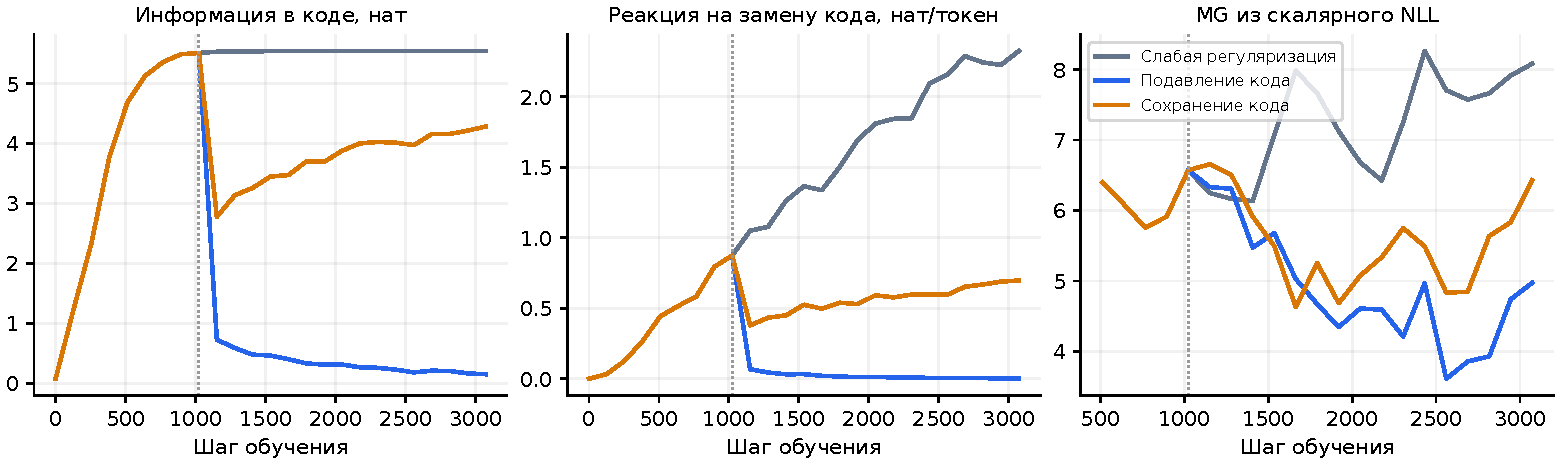
\includegraphics[width=\linewidth,height=.32\textheight,keepaspectratio]{trajectory_seed1.pdf}\end{center}

На рисунке показан первый проверочный сид, без выбора «самого красивого». Вертикальная линия --- разветвление на шаге 1024. MG получает только скалярный NLL; две левые панели не используются для его вычисления.

\textbf{Преимущество этого контроля.} При одинаковом внешнем весе KL метод различает две ветки с разной сохранностью латентной информации. Это усиливает интерпретацию MG как индикатора содержательного изменения обучения. Контроль не отделяет влияние всех деталей функции потерь и не доказывает причинную связь каждого колебания MG с MI.

\newpage
\section*{6. Воспроизводимость, окна и выбор наблюдаемого лога}

\begin{center}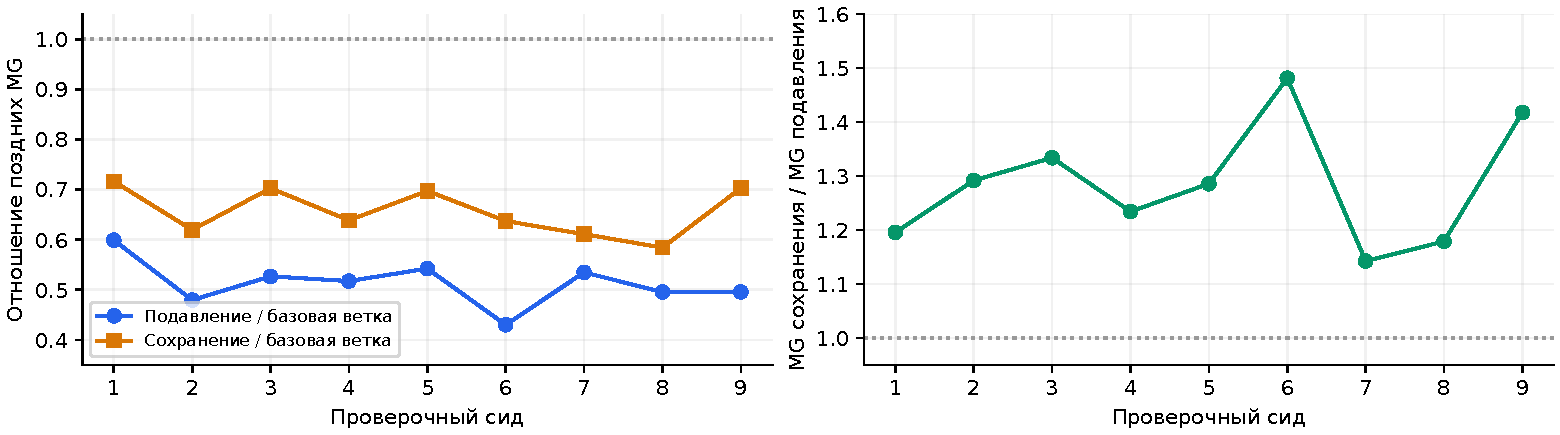
\includegraphics[width=\linewidth,height=.32\textheight,keepaspectratio]{seed_comparison.pdf}\end{center}

\begin{center}\small
\begin{tabularx}{\linewidth}{l>{\raggedright\arraybackslash}X>{\raggedright\arraybackslash}X>{\raggedright\arraybackslash}X}
\toprule
Окно / задержка & Подавление: медиана $q$ & Правильное направление & Сохранение: MG / подавление \\
\midrule
256 / 1 & 0.499 & 9/9 & 1.299; выше в 9/9 \\
512 / 1 (основная) & 0.517 & 9/9 & 1.286; выше в 9/9 \\
1024 / 1 & 0.536 & 9/9 & 1.254; выше в 9/9 \\
512 / 4 & 0.898 & 7/9 & 1.285; выше в 9/9 \\
\bottomrule\end{tabularx}\end{center}

При задержке 4 исключение Theiler также увеличивается до 156; это чувствительность совместной настройки, а не чистый эффект одной задержки. Для окна 1024 есть только одно раннее окно. Устойчивость к размеру окна подтверждена в проверенном диапазоне, устойчивость ко всем задержкам --- нет.

\textbf{Лог важен.} На обычном NLL случайного обучающего мини-батча парный MG изменился в нужную сторону лишь на 4/9 сидов; отношения лежат в диапазоне 0.973--1.028. Положительный результат относится к фиксированному контрольному батчу. Перенос на произвольный уже имеющийся loss-log не установлен.

\textbf{Сильные простые альтернативы.} Стандартное отклонение того же контрольного лога и его спектральная энтропия также различили подавление на 9/9 сидов. Для сохранения кода STD выросло на 9/9, энтропия --- на 7/9. Поэтому повторяемость результата MG доказана, а его уникальность относительно дешёвых статистик --- нет. Контроль умножением лога на 10 пройден; суррогаты IAAFT не установили особого преимущества нелинейной геометрии. В основных окнах не было вырождения, однако рекуррентность и абсолютная размерная интерпретация не подтверждены.

\section*{7. Циклический VAE: проверка практического мониторинга}

На новых инициализациях 100--109 после 1024 шагов разогрева проведены три цикла по 2048 обновлений: $\beta$ линейно растёт от 0 до 1 в первой половине и остаётся 1 во второй; затем сбрасывается. Всего 7168 шагов. Free bits здесь нет. MG не управляет обучением: по сохранённым логам воспроизводятся решения наблюдателя, использующего только прошлые данные.

Независимые проверки выполнялись каждые 64 шага. Событие потери --- обе диагностики не выше 50\% раннего уровня; восстановления --- обе не ниже 65\%. Требуются два последовательных подтверждения, время события --- второе из них. На девяти проверочных сидах получено \textbf{41 событие: 23 потери и 18 восстановлений} с полным горизонтом оценки 512 шагов; ещё два поздних события учитываются отдельно.

Наблюдатель запрашивает дорогую проверку при достаточно большом абсолютном изменении логарифма своего признака относительно последнего запроса, с паузой минимум 128 шагов. Пороги выбирались только на пилоте 100 из заранее заданной сетки и отдельно для бюджетов 6, 12, 24; основной бюджет --- 12. Все методы получают одну общую начальную проверку. Попадание засчитывается в пределах 512 шагов после подтверждения события и до противоположного перехода. Повторные проверки одного события не дают дополнительных попаданий.

\newpage
\section*{8. Где MG полезен, а где мониторинг пока проигрывает}

\begin{center}\small
\begin{tabularx}{\linewidth}{l>{\raggedright\arraybackslash}X>{\raggedright\arraybackslash}X>{\raggedright\arraybackslash}X}
\toprule
Метод назначения проверок & Бюджет 6: найдено / 41 & Бюджет 12: найдено / 41 & Бюджет 24: найдено / 41 \\
\midrule
MG & 18 & 28 & 36 \\
STD контрольного лога & 13 & 20 & 38 \\
Спектральная энтропия & 17 & 28 & 35 \\
KL из обучения & 8 & 13 & 31 \\
Изменение расписания $\beta$ & 18 & 18 & 26 \\
Равномерные проверки & 12 & 38 & 40 \\
\bottomrule\end{tabularx}\end{center}

При шести проверках MG находит больше событий, чем равномерная схема: 18 против 12, включая и потерю (8), и восстановление (10). Но тот же общий результат даёт расписание $\beta$ за счёт обнаружения восстановлений. При основном бюджете 12 MG находит 28/41, а периодические проверки --- 38/41. MG использует в среднем 9.4 запроса; даже при точно таком же числе запросов на каждом сиде периодическая схема находит 34 события. Разница средней по сидам полноты MG и основной периодической схемы --- \ensuremath{-}24.4 процентного пункта, 95\%-й bootstrap-интервал [\ensuremath{-}36.7; \ensuremath{-}10.0].

Следовательно, \textbf{связь MG с потерей информации подтверждена сильнее, чем выгода от его использования для назначения проверок}. На данном регулярном циклическом расписании преимущество по полноте мониторинга не показано.

\section*{9. Вычислительная стоимость: обработка и получение лога}

Последовательный прогретый CPU-бенчмарк: 40 чередующихся повторов, 2 потока PyTorch и 1 поток оценивателя. Медиана расчёта одного окна MG --- \textbf{12.89 мс}, комплексной проверки MI и замены кода --- \textbf{209.32 мс}, получения одного контрольного NLL --- 7.13 мс. Обработка уже записанного окна MG примерно \textbf{в 16.2 раза дешевле одной специализированной проверки}. Это сравнение операций, а не равной точности или сквозного ускорения мониторинга.

\begin{center}\small
\begin{tabularx}{\linewidth}{l>{\raggedright\arraybackslash}X>{\raggedright\arraybackslash}X}
\toprule
Затраты на запуск, бюджет 12 & С получением лога, с & Если нужный лог уже есть, с \\
\midrule
MG и запрошенные проверки & 54.68 & 3.54 \\
STD и запрошенные проверки & 53.86 & 2.73 \\
Энтропия и запрошенные проверки & 53.59 & 2.45 \\
KL и запрошенные проверки & 2.72 & 2.72 \\
Равномерные 12 + 1 проверки & 2.72 & 2.72 \\
Частые 96 + 1 проверки & 20.30 & 20.30 \\
\bottomrule\end{tabularx}\end{center}

Это расчёт из измеренных стоимостей операций и фактического числа запросов, усреднённого по девяти сидам, без стоимости самого обучения. Получение 7168 контрольных значений стоит около 51.14 с и доминирует. Для MG учтены 105 окон и запрошенные проверки, включая начальную. Оценочные эталонные измерения, нужные для разметки событий, не выдаются за эксплуатационную экономию. На машине могла идти сторонняя работа; параллельные времена обучения не используются для сравнения скорости.

\section*{10. Подтверждённые преимущества и вывод для статьи}

\textbf{Информативность одного скаляра:} MG отражает независимо установленную потерю информации без чтения скрытых представлений и без включения MI/KL в свой вход. \textbf{Воспроизводимость:} направление эффекта сохранено на 9/9 проверочных инициализаций и трёх размерах окна. \textbf{Содержательный контроль:} частичная защита кода сопровождается более высоким MG на тех же 9/9 сидах. \textbf{Небольшая стоимость обработки:} около 13 мс на окно уже доступного лога в локальном бенчмарке.

Подходящая формулировка для статьи: «В обучении текстового VAE оценка по скалярному логу реконструкции устойчиво отражает потерю латентной информации, подтверждённую взаимной информацией и реакцией декодера на замену кода. Контроль с сохранением информации и повторения по инициализациям поддерживают применение метода как индикатора изменений обучения».

Границы вывода: одна небольшая модель и один корпус; точное число активных компонент не установлено; ухудшение латентного представления не является улучшением модели. Превосходство над простыми статистиками, сквозное ускорение и перенос на LLM не показаны. Все ветки, неудачная защита encoder5, чувствительности и бюджеты включены в эту сводку; подробные числа и происхождение данных приложены в архиве.
\end{document}